\section{Mosaic matrices for categorical data}\label{sec:mosmat}

One reason for the wide usefulness of graphs of quantitative data
has been the
development of effective, general techniques for dealing with high-dimensional \Dsets.
The \scatmat{}
(\SSSGref{8.3.2})
shows all pairwise (marginal) views of a set of variables
in a coherent display, whose design goal is to show the interdependence
among the collection of variables as a whole.
It combines multiple views of the data
into a single display which allows detection of patterns which could
not readily be discerned from a series of separate graphs.
In effect, a multivariate \Dset\ in $p$ dimensions (variables) is shown as
a collection of $p (p-1)$ two-dimensional \scats{}, each of which is
the projection of the cloud of points on two of the variable axes.
These ideas can be readily extended to categorical data.

A \mway{} \ctab{} of $p$ categorical variables,
$A, B, C,\dots$, also contains the interdependence among the collection
of variables as a whole.  The saturated \loglin{} model, $[A B C\dots]$
fits this interdependence perfectly, but is often too complex to describe
or understand.  By summing the table over all variables except two,
$A$ and $B$, say, we obtain a two-variable (marginal) table, showing the
bivariate relationship between $A$ and $B$, which is also a projection
of the $p$-variable relation into the space of two (categorical) variables.
If we do this for all $p (p-1)$ unordered pairs of categorical variables
and display each two-variable table as a mosaic,  we have a categorical
analog of the \scatmat{}, called a
\glossterm{mosaic matrix}.
Like the \scatmat{}, the mosaic matrix can accommodate any number of
variables in principle, but in practice is limited by the resolution
of our display to three or four variables.

Mosaic matrices are produced using the \IML{}
module \texttt{mosmat}, which is called in a \PROC{IML} step as
\begin{listing}
   run mosmat(dim, table, vnames, lnames, plots, title);
\end{listing}
When there are $p$ variables in the \texttt{table}, a set of $p^2$ plots
are produced;  these include the $p (p-1)$ pairwise mosaics and a set
of $p$ panels containing the variable names (from \texttt{vnames}).
After the \IML{} step, the separate plots may be combined into one figure with the \macro{PANELS}.
The \macro{MOSMAT} provides a simple interface to these steps.

\begin{Example}[marital2]{Marital status and pre- and extramarital sex}
In \exref{ex:marital1} we examined a series of models relating marital
status to reported premarital and extramarital sexual activity and gender.
\figref{fig:mosmat5} shows the mosaic matrix for these data,
produced with the \macro{MOSMAT}, as follows:
\begin{listing}
%include catdata(marital);
%mosmat(data=marital, var=Gender Pre Extra Marital,
   vorder=Marital Extra Pre Gender, devtype=LR ADJ);
\end{listing}

If we view gender, premarital sex and extramarital sex as explanatory,
and marital status (divorced vs.\  still married) as the response,
then the mosaics in row 1 (and in column 1)%
%
\footnote{Rows and columns in the mosaic matrix are identified
as in a table or numerical matrix, with row 1, column 1 in the upper left corner.}
%
shows how marital status
depends on each predictor marginally.
The remaining panels show the relations within the set of explanatory
variables.

%% one figure
\begin{figure}[htb]
  \centering
  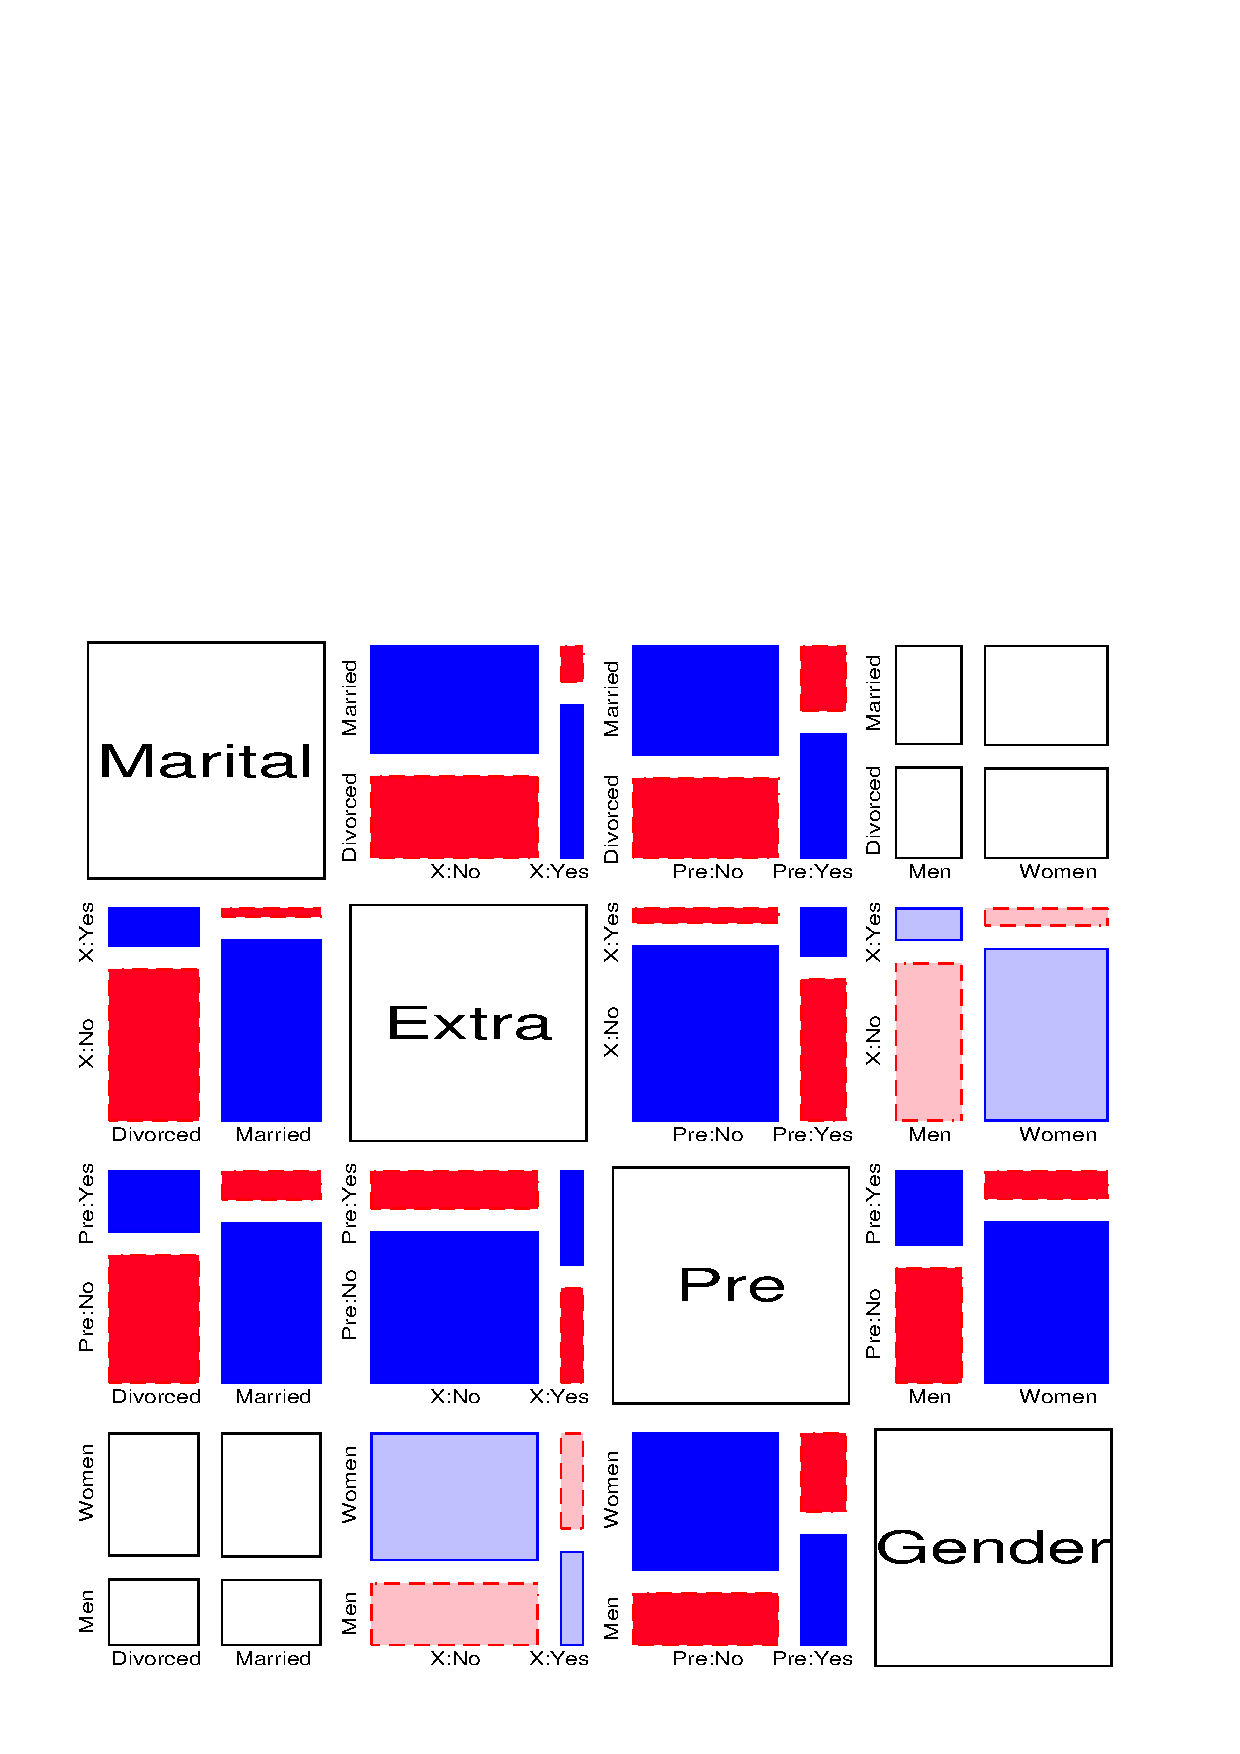
\includegraphics[scale=.8]{ch4/fig/mosmat5m}
  \caption[Mosaic matrix for marital status data]{Mosaic matrix for marital status data.
  Each panel shows the marginal relation,
fitting an independence model between the row and column variable, collapsed over other variable(s).}%
  \label{fig:mosmat5}
\end{figure}

Thus, we see in row 1, column 4, that marital status is independent
of gender (all residuals equal zero, here), by design of the data
collection.  In the (1, 3) panel, we see that reported premarital sex
is more often followed by divorce, while non-report is more prevalent
among those still married.  The (1, 2) panel shows a similar, but stronger relation between extramarital sex and marriage stability.  These
effects pertain to the associations of P and E with marital status---%
the terms [PM] and [EM] in the \loglin{} model.  We saw earlier that
an interaction of P and E (the term [PEM]) is required to fully account for these data.  This effect is not displayed in \figref{fig:mosmat5}.

Among the background variables (the \loglin{} term [GPE]), the (2, 3) panel shows a strong relation
between premarital sex and subsequent extramarital sex, while
the (2, 4) and (3, 4) panels show that men are far more likely to report
premarital sex than women in this sample, and also more likely to
report extramarital sex.
\end{Example}

\begin{Example}[berkeley4]{Berkeley admissions}
\figref{fig:mosmat9a} shows the pairwise marginal
relations among the variables
Admit, Gender and Department in the Berkeley
data which were examined earlier (\exref{ex:berkeley1}) in fourfold displays
(\figref{fig:fourfold13} and \figref{fig:pie2x2b}).
This figure is produced using the \macro{MOSMAT} as shown below.
The \macro{TABLE} is first used to recode the factor variables
to more meaningful character labels.
%% input: /Users/friendly/sasuser/mosaics/mosmat9m.sas
%% last modified: 19-Jul-99 10:44
\begin{listing}
%include goptions;
goptions hsize=7 in vsize=7 in;
libname mosaic '~/sasuser/mosaics';
 
%include catdata(berkeley);
proc format;
   value admit 1="Admit" 0="Reject" ;
   value dept  1="A" 2="B" 3="C" 4="D" 5="E" 6="F";
   value $sex  'M'='Male'   'F'='Female';
%table(data=berkeley, var=Admit Gender Dept, weight=freq, char=Y,
        format=admit admit. gender $sex. dept dept., 
        order=data, out=berkeley);

%mosmat(data=berkeley, vorder=Admit Gender Dept, sort=no, htext=3.5);
\end{listing}


The panel in row 2, column 1
shows that Admission and Gender are
strongly associated marginally, as we saw in \figref{fig:fourfold13},
and overall, males are more often admitted.
The diagonally-opposite panel (row 1, column 2) shows the
same relation, splitting first by gender.%
%
\footnote{Note that this is different than just the transpose or interchange
of horizontal and vertical dimensions as in the \scatmat{},
because the mosaic display splits the total frequency first by the horizontal
variable and then (conditionally) by the vertical variable.
The areas of all corresponding tiles are the same in each diagonally
opposite pair, however, as are the
residuals shown by color and shading.}
%
\begin{figure}[!htb]
  \centering
  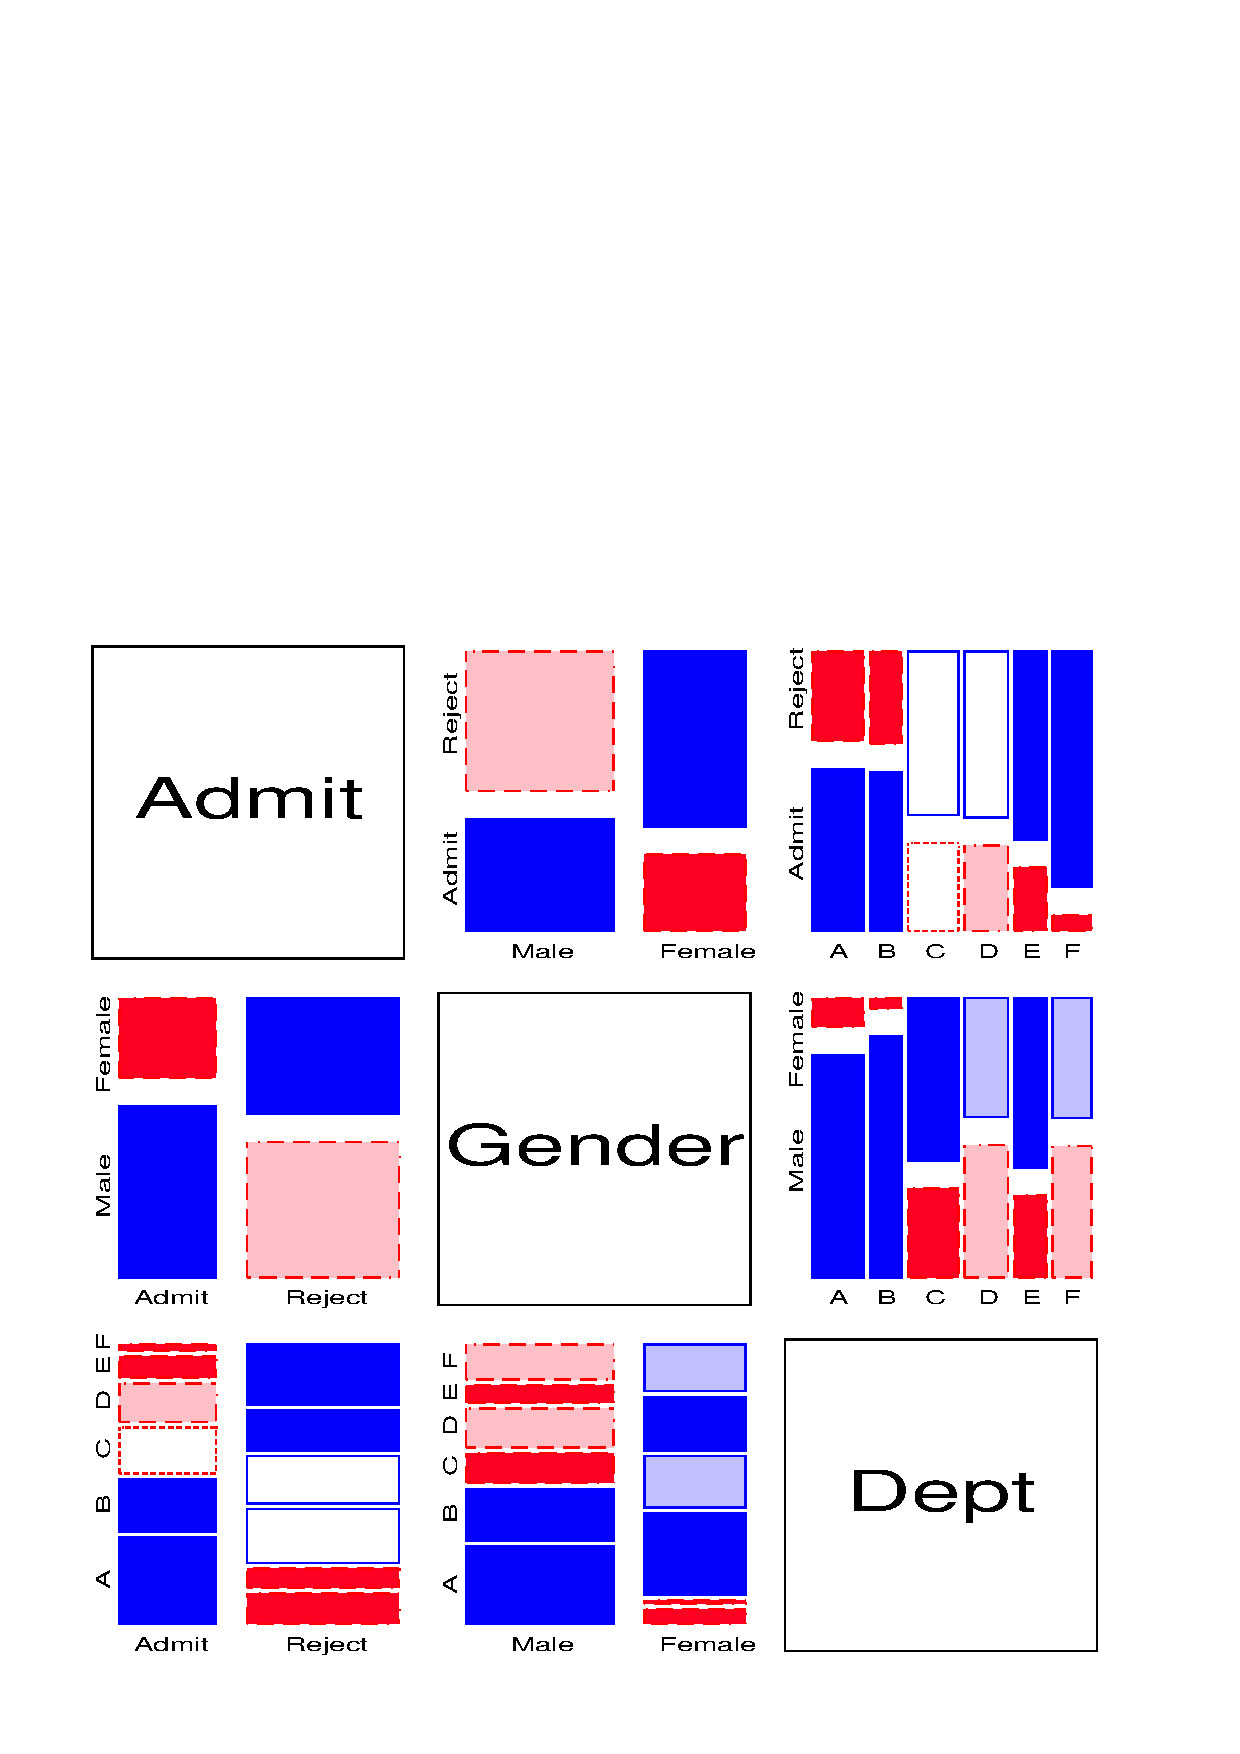
\includegraphics[scale=.8]{ch4/fig/mosmat9a}
  \caption[Marginal mosaic matrix of Berkeley
admissions]{Mosaic matrix of Berkeley
admissions, showing bivariate marginal relations.}\label{fig:mosmat9a}
\end{figure}

The panels in the third column (and third row)
illuminate the explanation for the paradoxical
result (see \figref{fig:pie2x2b}) that, within all but department A,
the likelihood of admission is equal for men and women,
yet, overall, there appears to be a bias in favor of admitting men
(see \figref{fig:fourfold13}).
The (1,3) and (3, 1) panels show
the marginal relation between Admission and Department; departments A and B have the greatest
overall admission rate, departments E and F the least.
The (2, 3) panel shows that men apply in much greater numbers to
departments A and B, while women apply in greater numbers to
the departments with the lowest overall rate of admission.
\end{Example}

\subsection{Conditional mosaic matrices}\label{sec:condmat}

We need not show the marginal relation between
each pair of variables in the mosaic matrix.
A conditional mosaic matrix fits a model of conditional independence
between each row and column, controlling for one or more of the other
variables.   \citet{Friendly:99b} gives further details and describes
analogous displays for quantitative data.

\begin{Example}[berkeley4b]{Berkeley admissions}
For example, \figref{fig:mosmat9b} shows all pairwise \emph{conditional}
relations among the variables Gender, Dept, Admit in the Berkeley data.
All panels show the \emph{same} observed frequencies in the three-way table
by the areas of the tiles,
but each fits a model of conditional independence between the row and
column variable, with the remaining variable controlled.
Thus, the shading in the (1,2) and (2,1) panels show the fit of the model
[Admit, Dept] [Gender, Dept],
which asserts that Admission and Gender are independent, given (controlling
for) Department.  Except for Department A, this model fits quite well,
again indicating lack of gender bias.
The (1,3) and (3,1) panels show the relation between admission and department
controlling for gender, highlighting the differential admission rates
across departments.
\begin{figure}[!htb]
  \centering
  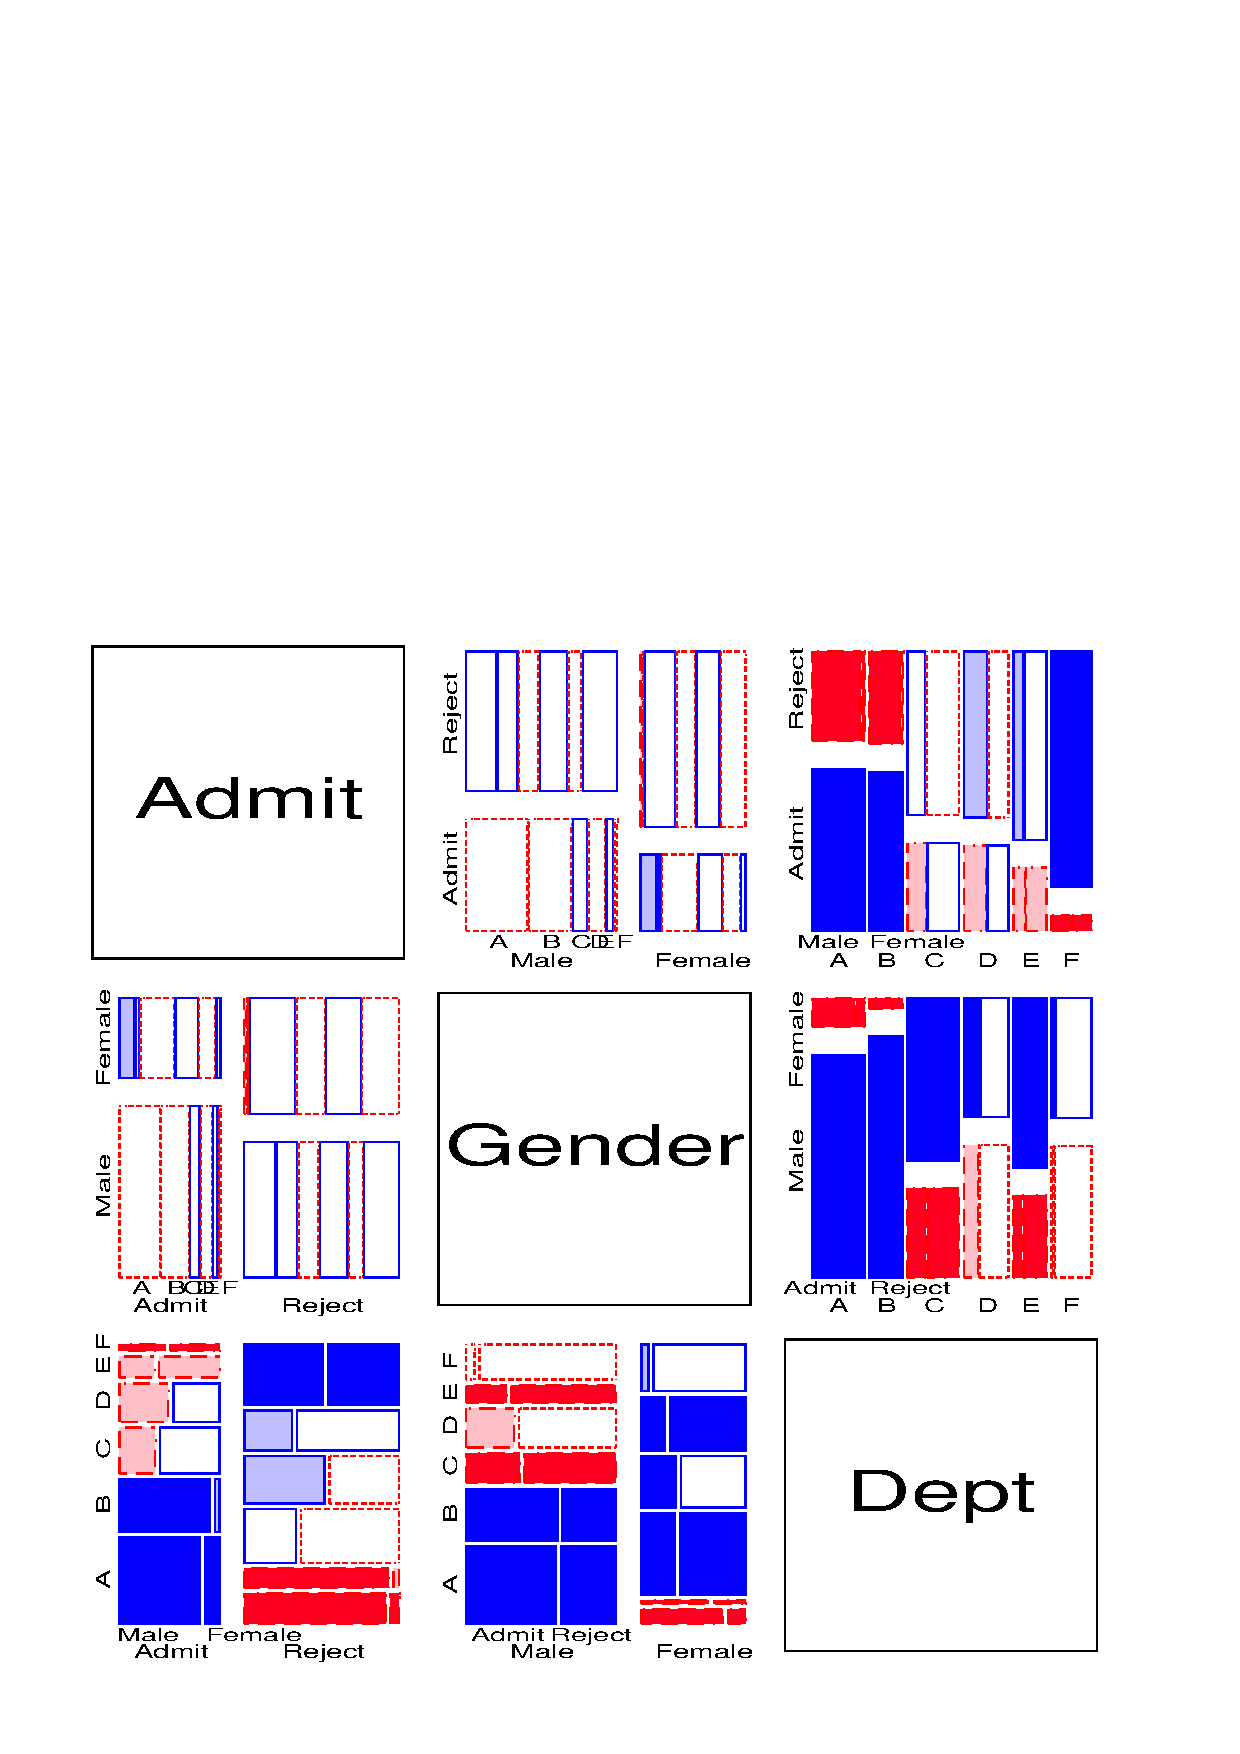
\includegraphics[scale=.8]{ch4/fig/mosmat9b}
  \caption[Conditional mosaic matrix of Berkeley
admissions]{Conditional mosaic matrix of Berkeley
admissions.  Each panel shows the conditional relation,
fitting a model of conditional independence between the row and column variable, controlling for other variable(s).}\label{fig:mosmat9b}
\end{figure}

Conditional mosaic matrices are produced with the \macro{MOSMAT}
by specifying \texttt{CONDIT} as the \mparm{fittype}{MOSMAT}.
The parameter \texttt{plots=3} specifies that each panel in the
display contains the three-way mosaic plot for the data.
%% input: /Users/friendly/sasuser/mosaics/mosmat9m.sas
%% last modified: 19-Jul-99 10:44
\begin{listing}
%mosmat(data=berkeley, vorder=Admit Gender Dept, sort=no, htext=3.5,
   plots=3, fittype=CONDIT);
\end{listing}

\end{Example}
